
%% We use the memoir class because it offers a many easy to use features.
\documentclass[10pt,a4paper,titlepage,openany,oneside]{memoir}

%% `usepackage` commands.
%% Packages
%% ========

%% LaTeX Font encoding -- DO NOT CHANGE
\usepackage[OT1]{fontenc}

%% Babel provides support for languages.  'english' uses British
%% English hyphenation and text snippets like "Figure" and
%% "Theorem". Use the option 'ngerman' if your document is in German.
%% Use 'american' for American English.  Note that if you change this,
%% the next LaTeX run may show spurious errors.  Simply run it again.
%% If they persist, remove the .aux file and try again.
\usepackage[english]{babel}

%% Input encoding 'utf8'. In some cases you might need 'utf8x' for
%% extra symbols. Not all editors, especially on Windows, are UTF-8
%% capable, so you may want to use 'latin1' instead.
\usepackage[utf8]{inputenc}

%% This changes default fonts for both text and math mode to use Herman Zapfs
%% excellent Palatino font. Do not change this.
\usepackage[sc]{mathpazo}

%% The AMS-LaTeX extensions for mathematical typesetting.  Do not
%% remove.
\usepackage{amsmath,amssymb,amsfonts,mathrsfs}
\allowdisplaybreaks

%% NTheorem is a reimplementation of the AMS Theorem package. This
%% will allow us to typeset theorems like examples, proofs and
%% similar.  Do not remove.
%% NOTE: Must be loaded AFTER amsmath, or the \qed placement will
%% break
\usepackage[amsmath,thmmarks]{ntheorem}

%% LaTeX' own graphics handling
\usepackage{graphicx}

%% We unfortunately need this for the Rules chapter.  Remove it
%% afterwards; or at least NEVER use its underlining features.
\usepackage{soul}

%% This allows you to add .pdf files. It is used to add the
%% declaration of originality.
\usepackage{pdfpages}

%% Extra Packages
%% ==============

%% [OPT] Multi-rowed cells in tabulars
%\usepackage{multirow}

%% [REC] Intelligent cross reference package. This allows for nice
%% combined references that include the reference and a hint to where
%% to look for it.
\usepackage{varioref}

%% [OPT] Easily changeable quotes with \enquote{Text}
%\usepackage[german=swiss]{csquotes}

%% [REC] Format dates and time depending on locale
\usepackage{datetime}

%% [OPT] Provides a \cancel{} command to stroke through mathematics.
%\usepackage{cancel}

%% [NEED] This allows for additional typesetting tools in mathmode.
%% See its excellent documentation.
\usepackage{mathtools}

%% [ADV] Conditional commands
%\usepackage{ifthen}

%% [OPT] Manual large braces or other delimiters.
%\usepackage{bigdelim, bigstrut}

%% [REC] Alternate vector arrows. Use the command \vv{} to get scaled
%% vector arrows.
\usepackage[h]{esvect}

%% [NEED] Some extensions to tabulars and array environments.
\usepackage{array}

%% [OPT] Postscript support via pstricks graphics package. Very
%% diverse applications.
%\usepackage{pstricks,pst-all}

%% [?] This seems to allow us to define some additional counters.
%\usepackage{etex}

%% [ADV] XY-Pic to typeset some matrix-style graphics
%\usepackage[all]{xy}

%% [OPT] This is needed to generate an index at the end of the
%% document.
%\usepackage{makeidx}

%% [OPT] Fancy package for source code listings.  The template text
%% needs it for some LaTeX snippets; remove/adapt the \lstset when you
%% remove the template content.
\usepackage{listings}
\lstset{language=TeX,basicstyle={\normalfont\ttfamily}}

%% [REC] Fancy character protrusion.  Must be loaded after all fonts.
\usepackage[activate]{pdfcprot}

%% [REC] Nicer tables.  Read the excellent documentation.
\usepackage{booktabs}

%% Fancy Enumeration environment
\usepackage{enumitem}

%% Bibliography package.
\usepackage[
style=authoryear,
sorting=ynt,
natbib=true,
mincitenames=1,
maxcitenames=2,
backend=biber]{biblatex}
\addbibresource{reference.bib}

%% Side-by-Side Figures
\usepackage{caption}
\usepackage{subcaption}

%% Bold math symbols.
\usepackage{bm}
\usepackage{bbm}

%% Color for table cells.
\usepackage{xcolor,colortbl}

%% Table multiple rows.
\usepackage{multirow}

%% Algorithms environment
\usepackage[ruled,vlined,linesnumbered,noresetcount]{algorithm2e}

%% Force Figures to not float out of Section
\usepackage{float}

%% API
%% ===

%% Make document internal hyperlinks wherever possible. (TOC, references)
%% This MUST be loaded after varioref. We just load it last to be safe.
\usepackage[
linkcolor=black,
colorlinks=true,
citecolor=black,
filecolor=black]{hyperref}

% \let\oldcitet=\citet
% \let\oldcitep=\citep 
% \renewcommand{\citet}[1]{\textcolor[rgb]{0,0,1}{\oldcitet{#1}}}
% \renewcommand{\citep}[1]{\textcolor[rgb]{0,0,1}{\oldcitep{#1}}}


%% Memoir layout setup

%% NOTE: You are strongly advised not to change any of them unless you
%% know what you are doing.  These settings strongly interact in the
%% final look of the document.

% Turn extra space before chapter headings off.
\setlength{\beforechapskip}{0pt}

\nonzeroparskip
\parindent=0pt
\defaultlists

% Chapter style redefinition
\makeatletter

\if@twoside
  \pagestyle{Ruled}
  \copypagestyle{chapter}{Ruled}
\else
  \pagestyle{ruled}
  \copypagestyle{chapter}{ruled}
\fi
\makeoddhead{chapter}{}{}{}
\makeevenhead{chapter}{}{}{}
\makeheadrule{chapter}{\textwidth}{0pt}
\copypagestyle{abstract}{empty}

\makechapterstyle{bianchimod}{%
  \chapterstyle{default}
  \renewcommand*{\chapnamefont}{\normalfont\Large\sffamily}
  \renewcommand*{\chapnumfont}{\normalfont\Large\sffamily}
  \renewcommand*{\printchaptername}{%
    \chapnamefont\centering\@chapapp}
  \renewcommand*{\printchapternum}{\chapnumfont {\thechapter}}
  \renewcommand*{\chaptitlefont}{\normalfont\huge\sffamily}
  \renewcommand*{\printchaptertitle}[1]{%
    \hrule\vskip\onelineskip \centering \chaptitlefont\textbf{\vphantom{gyM}##1}\par}
  \renewcommand*{\afterchaptertitle}{\vskip\onelineskip \hrule\vskip
    \afterchapskip}
  \renewcommand*{\printchapternonum}{%
    \vphantom{\chapnumfont {9}}\afterchapternum}}

% Use the newly defined style
\chapterstyle{bianchimod}

\setsecheadstyle{\Large\bfseries\sffamily}
\setsubsecheadstyle{\large\bfseries\sffamily}
\setsubsubsecheadstyle{\bfseries\sffamily}
\setparaheadstyle{\normalsize\bfseries\sffamily}
\setsubparaheadstyle{\normalsize\itshape\sffamily}
\setsubparaindent{0pt}

% Set captions to a more separated style for clearness
\captionnamefont{\sffamily\bfseries\footnotesize}
\captiontitlefont{\sffamily\footnotesize}
\setlength{\intextsep}{12pt}
\setlength{\belowcaptionskip}{1pt}

% Set section and TOC numbering depth to subsection
\setsecnumdepth{subsection}
\settocdepth{subsection}

%% Titlepage adjustments
\pretitle{\vspace{0pt plus 0.7fill}\begin{center}\HUGE\sffamily\bfseries}
\posttitle{\end{center}\par}
\preauthor{\par\begin{center}\let\and\\\Large\sffamily}
\postauthor{\end{center}}
\predate{\par\begin{center}\Large\sffamily}
\postdate{\end{center}}

\def\@advisors{}
\newcommand{\advisors}[1]{\def\@advisors{#1}}
\def\@department{}
\newcommand{\department}[1]{\def\@department{#1}}
\def\@thesistype{}
\newcommand{\thesistype}[1]{\def\@thesistype{#1}}

\renewcommand{\maketitlehooka}{\noindent\logo[2.5in]}

\renewcommand{\maketitlehookb}{\vspace{1in}%
  \par\begin{center}\Large\sffamily\@thesistype\end{center}}

\renewcommand{\maketitlehookd}{%
  \vfill\par
  \begin{flushright}
    \sffamily
    \@advisors\par
    \@department, Imperial College London
  \end{flushright}
}

\checkandfixthelayout

\setlength{\droptitle}{-35pt} %-48

\makeatother

% This defines how theorems should look. Best leave as is.
\theoremstyle{plain}
\setlength\theorempostskipamount{0pt}

%%% Local Variables:
%%% mode: latex
%%% TeX-master: "thesis"
%%% End:



%% Theorem-like environments

\numberwithin{equation}{chapter}

%% English variants
\newtheorem{theorem}{Theorem}[chapter]
\newtheorem{example}[theorem]{Example}
\newtheorem{remark}[theorem]{Remark}
\newtheorem{corollary}[theorem]{Corollary}
\newtheorem{definition}[theorem]{Definition}
\newtheorem{lemma}[theorem]{Lemma}
\newtheorem{proposition}[theorem]{Proposition}
\newtheorem{hypothesis}[theorem]{Hypothesis}
\newtheorem{assumption}[theorem]{Assumption}

%% Proof environment with a small square as a "qed" symbol
\theoremstyle{nonumberplain}
\theorembodyfont{\normalfont}
\theoremsymbol{\ensuremath{\square}}
\newtheorem{proof}{Proof}
%\newtheorem{beweis}{Beweis}





%% Helpful macros.
%% Custom commands
%% ===============

%% logo command
\newcommand{\logo}[1][\textwidth]{\resizebox{#1}{!}{
\includegraphics{setup/logo}}}

%% Ian Goodfellow LaTeX commands for math.
%%%%% NEW MATH DEFINITIONS %%%%%



\def\ceil#1{\lceil #1 \rceil}
\def\floor#1{\lfloor #1 \rfloor}
\def\1{\bm{1}}
\newcommand{\train}{\mathcal{D}}
\newcommand{\valid}{\mathcal{D_{\mathrm{valid}}}}
\newcommand{\test}{\mathcal{D_{\mathrm{test}}}}

\def\eps{{\epsilon}}


% Random variables
\def\reta{{\textnormal{$\eta$}}}
\def\ra{{\textnormal{a}}}
\def\rb{{\textnormal{b}}}
\def\rc{{\textnormal{c}}}
\def\rd{{\textnormal{d}}}
\def\re{{\textnormal{e}}}
\def\rf{{\textnormal{f}}}
\def\rg{{\textnormal{g}}}
\def\rh{{\textnormal{h}}}
\def\ri{{\textnormal{i}}}
\def\rj{{\textnormal{j}}}
\def\rk{{\textnormal{k}}}
\def\rl{{\textnormal{l}}}
%\def\rm{{\textnormal{m}}}
\def\rn{{\textnormal{n}}}
\def\ro{{\textnormal{o}}}
\def\rp{{\textnormal{p}}}
\def\rq{{\textnormal{q}}}
\def\rr{{\textnormal{r}}}
\def\rs{{\textnormal{s}}}
\def\rt{{\textnormal{t}}}
\def\ru{{\textnormal{u}}}
\def\rv{{\textnormal{v}}}
\def\rw{{\textnormal{w}}}
\def\rx{{\textnormal{x}}}
\def\ry{{\textnormal{y}}}
\def\rz{{\textnormal{z}}}

% Random vectors
\def\rvepsilon{{\mathbf{\epsilon}}}
\def\rvtheta{{\mathbf{\theta}}}
\def\rva{{\mathbf{a}}}
\def\rvb{{\mathbf{b}}}
\def\rvc{{\mathbf{c}}}
\def\rvd{{\mathbf{d}}}
\def\rve{{\mathbf{e}}}
\def\rvf{{\mathbf{f}}}
\def\rvg{{\mathbf{g}}}
\def\rvh{{\mathbf{h}}}
\def\rvu{{\mathbf{i}}}
\def\rvj{{\mathbf{j}}}
\def\rvk{{\mathbf{k}}}
\def\rvl{{\mathbf{l}}}
\def\rvm{{\mathbf{m}}}
\def\rvn{{\mathbf{n}}}
\def\rvo{{\mathbf{o}}}
\def\rvp{{\mathbf{p}}}
\def\rvq{{\mathbf{q}}}
\def\rvr{{\mathbf{r}}}
\def\rvs{{\mathbf{s}}}
\def\rvt{{\mathbf{t}}}
\def\rvu{{\mathbf{u}}}
\def\rvv{{\mathbf{v}}}
\def\rvw{{\mathbf{w}}}
\def\rvx{{\mathbf{x}}}
\def\rvy{{\mathbf{y}}}
\def\rvz{{\mathbf{z}}}

% Elements of random vectors
\def\erva{{\textnormal{a}}}
\def\ervb{{\textnormal{b}}}
\def\ervc{{\textnormal{c}}}
\def\ervd{{\textnormal{d}}}
\def\erve{{\textnormal{e}}}
\def\ervf{{\textnormal{f}}}
\def\ervg{{\textnormal{g}}}
\def\ervh{{\textnormal{h}}}
\def\ervi{{\textnormal{i}}}
\def\ervj{{\textnormal{j}}}
\def\ervk{{\textnormal{k}}}
\def\ervl{{\textnormal{l}}}
\def\ervm{{\textnormal{m}}}
\def\ervn{{\textnormal{n}}}
\def\ervo{{\textnormal{o}}}
\def\ervp{{\textnormal{p}}}
\def\ervq{{\textnormal{q}}}
\def\ervr{{\textnormal{r}}}
\def\ervs{{\textnormal{s}}}
\def\ervt{{\textnormal{t}}}
\def\ervu{{\textnormal{u}}}
\def\ervv{{\textnormal{v}}}
\def\ervw{{\textnormal{w}}}
\def\ervx{{\textnormal{x}}}
\def\ervy{{\textnormal{y}}}
\def\ervz{{\textnormal{z}}}

% Random matrices
\def\rmA{{\mathbf{A}}}
\def\rmB{{\mathbf{B}}}
\def\rmC{{\mathbf{C}}}
\def\rmD{{\mathbf{D}}}
\def\rmE{{\mathbf{E}}}
\def\rmF{{\mathbf{F}}}
\def\rmG{{\mathbf{G}}}
\def\rmH{{\mathbf{H}}}
\def\rmI{{\mathbf{I}}}
\def\rmJ{{\mathbf{J}}}
\def\rmK{{\mathbf{K}}}
\def\rmL{{\mathbf{L}}}
\def\rmM{{\mathbf{M}}}
\def\rmN{{\mathbf{N}}}
\def\rmO{{\mathbf{O}}}
\def\rmP{{\mathbf{P}}}
\def\rmQ{{\mathbf{Q}}}
\def\rmR{{\mathbf{R}}}
\def\rmS{{\mathbf{S}}}
\def\rmT{{\mathbf{T}}}
\def\rmU{{\mathbf{U}}}
\def\rmV{{\mathbf{V}}}
\def\rmW{{\mathbf{W}}}
\def\rmX{{\mathbf{X}}}
\def\rmY{{\mathbf{Y}}}
\def\rmZ{{\mathbf{Z}}}

% Elements of random matrices
\def\ermA{{\textnormal{A}}}
\def\ermB{{\textnormal{B}}}
\def\ermC{{\textnormal{C}}}
\def\ermD{{\textnormal{D}}}
\def\ermE{{\textnormal{E}}}
\def\ermF{{\textnormal{F}}}
\def\ermG{{\textnormal{G}}}
\def\ermH{{\textnormal{H}}}
\def\ermI{{\textnormal{I}}}
\def\ermJ{{\textnormal{J}}}
\def\ermK{{\textnormal{K}}}
\def\ermL{{\textnormal{L}}}
\def\ermM{{\textnormal{M}}}
\def\ermN{{\textnormal{N}}}
\def\ermO{{\textnormal{O}}}
\def\ermP{{\textnormal{P}}}
\def\ermQ{{\textnormal{Q}}}
\def\ermR{{\textnormal{R}}}
\def\ermS{{\textnormal{S}}}
\def\ermT{{\textnormal{T}}}
\def\ermU{{\textnormal{U}}}
\def\ermV{{\textnormal{V}}}
\def\ermW{{\textnormal{W}}}
\def\ermX{{\textnormal{X}}}
\def\ermY{{\textnormal{Y}}}
\def\ermZ{{\textnormal{Z}}}

% Vectors
\def\vzero{{\bm{0}}}
\def\vone{{\bm{1}}}
\def\va{{\bm{a}}}
\def\vb{{\bm{b}}}
\def\vc{{\bm{c}}}
\def\vd{{\bm{d}}}
\def\ve{{\bm{e}}}
\def\vf{{\bm{f}}}
\def\vg{{\bm{g}}}
\def\vh{{\bm{h}}}
\def\vi{{\bm{i}}}
\def\vj{{\bm{j}}}
\def\vk{{\bm{k}}}
\def\vl{{\bm{l}}}
\def\vm{{\bm{m}}}
\def\vn{{\bm{n}}}
\def\vo{{\bm{o}}}
\def\vp{{\bm{p}}}
\def\vq{{\bm{q}}}
\def\vr{{\bm{r}}}
\def\vs{{\bm{s}}}
\def\vt{{\bm{t}}}
\def\vu{{\bm{u}}}
\def\vv{{\bm{v}}}
\def\vw{{\bm{w}}}
\def\vx{{\bm{x}}}
\def\vy{{\bm{y}}}
\def\vz{{\bm{z}}}
\def\vlambda{{\bm{\lambda}}}
\def\vmu{{\bm{\mu}}}
\def\valpha{{\bm{\alpha}}}
\def\vbeta{{\bm{\beta}}}
\def\vgamma{{\bm{\gamma}}}
\def\vtheta{{\bm{\theta}}}
\def\vepsilon{{\bm{\epsilon}}}
\def\vomega{{\bm{\omega}}}
\def\vpsi{{\bm{\psi}}}
\def\vphi{{\bm{\phi}}}
\def\vsigma{{\bm{\sigma}}}
\def\vSigma{{\bm{\Sigma}}}
\def\veta{{\bm{\eta}}}
\def\vrho{{\bm{\rho}}}
\def\vRho{{\bm{\Rho}}}
\def\vphi{{\bm{\phi}}}
\def\vPhi{{\bm{\Phi}}}
\def\vDelta{{\bm{\Delta}}}
\def\vdelta{{\bm{\delta}}}

%\def\KeyIdea{{\marginpar{KEY IDEA}}}
% YB: until we populate the book more thoroughly with KEY IDEA, probably best to leave this out
\def\KeyIdea{}

% Elements of vectors
\def\evalpha{{\alpha}}
\def\evbeta{{\beta}}
\def\evepsilon{{\epsilon}}
\def\evlambda{{\lambda}}
\def\evomega{{\omega}}
\def\evmu{{\mu}}
\def\evpsi{{\psi}}
\def\evsigma{{\sigma}}
\def\evtheta{{\theta}}
\def\eva{{a}}
\def\evb{{b}}
\def\evc{{c}}
\def\evd{{d}}
\def\eve{{e}}
\def\evf{{f}}
\def\evg{{g}}
\def\evh{{h}}
\def\evi{{i}}
\def\evj{{j}}
\def\evk{{k}}
\def\evl{{l}}
\def\evm{{m}}
\def\evn{{n}}
\def\evo{{o}}
\def\evp{{p}}
\def\evq{{q}}
\def\evr{{r}}
\def\evs{{s}}
\def\evt{{t}}
\def\evu{{u}}
\def\evv{{v}}
\def\evw{{w}}
\def\evx{{x}}
\def\evy{{y}}
\def\evz{{z}}

% Matrix
\def\mA{{\bm{A}}}
\def\mB{{\bm{B}}}
\def\mC{{\bm{C}}}
\def\mD{{\bm{D}}}
\def\mE{{\bm{E}}}
\def\mF{{\bm{F}}}
\def\mG{{\bm{G}}}
\def\mH{{\bm{H}}}
\def\mI{{\bm{I}}}
\def\mJ{{\bm{J}}}
\def\mK{{\bm{K}}}
\def\mL{{\bm{L}}}
\def\mM{{\bm{M}}}
\def\mN{{\bm{N}}}
\def\mO{{\bm{O}}}
\def\mP{{\bm{P}}}
\def\mQ{{\bm{Q}}}
\def\mR{{\bm{R}}}
\def\mS{{\bm{S}}}
\def\mT{{\bm{T}}}
\def\mU{{\bm{U}}}
\def\mV{{\bm{V}}}
\def\mW{{\bm{W}}}
\def\mX{{\bm{X}}}
\def\mY{{\bm{Y}}}
\def\mZ{{\bm{Z}}}
\def\mBeta{{\bm{\beta}}}
\def\mPhi{{\bm{\Phi}}}
\def\mLambda{{\bm{\Lambda}}}
\def\mSigma{{\bm{\Sigma}}}

% Tensor
% Got this from here: http://tex.stackexchange.com/questions/77640/bold-italic-and-sans-serif-math-symbols
\DeclareMathAlphabet{\mathsfit}{\encodingdefault}{\sfdefault}{m}{sl}
\SetMathAlphabet{\mathsfit}{bold}{\encodingdefault}{\sfdefault}{bx}{n}
\newcommand{\tens}[1]{\bm{\mathsfit{#1}}}
\def\tA{{\tens{A}}}
\def\tB{{\tens{B}}}
\def\tC{{\tens{C}}}
\def\tD{{\tens{D}}}
\def\tE{{\tens{E}}}
\def\tF{{\tens{F}}}
\def\tG{{\tens{G}}}
\def\tH{{\tens{H}}}
\def\tI{{\tens{I}}}
\def\tJ{{\tens{J}}}
\def\tK{{\tens{K}}}
\def\tL{{\tens{L}}}
\def\tM{{\tens{M}}}
\def\tN{{\tens{N}}}
\def\tO{{\tens{O}}}
\def\tP{{\tens{P}}}
\def\tQ{{\tens{Q}}}
\def\tR{{\tens{R}}}
\def\tS{{\tens{S}}}
\def\tT{{\tens{T}}}
\def\tU{{\tens{U}}}
\def\tV{{\tens{V}}}
\def\tW{{\tens{W}}}
\def\tX{{\tens{X}}}
\def\tY{{\tens{Y}}}
\def\tZ{{\tens{Z}}}


% Graph
\def\gA{{\mathcal{A}}}
\def\gB{{\mathcal{B}}}
\def\gC{{\mathcal{C}}}
\def\gD{{\mathcal{D}}}
\def\gE{{\mathcal{E}}}
\def\gF{{\mathcal{F}}}
\def\gG{{\mathcal{G}}}
\def\gH{{\mathcal{H}}}
\def\gI{{\mathcal{I}}}
\def\gJ{{\mathcal{J}}}
\def\gK{{\mathcal{K}}}
\def\gL{{\mathcal{L}}}
\def\gM{{\mathcal{M}}}
\def\gN{{\mathcal{N}}}
\def\gO{{\mathcal{O}}}
\def\gP{{\mathcal{P}}}
\def\gQ{{\mathcal{Q}}}
\def\gR{{\mathcal{R}}}
\def\gS{{\mathcal{S}}}
\def\gT{{\mathcal{T}}}
\def\gU{{\mathcal{U}}}
\def\gV{{\mathcal{V}}}
\def\gW{{\mathcal{W}}}
\def\gX{{\mathcal{X}}}
\def\gY{{\mathcal{Y}}}
\def\gZ{{\mathcal{Z}}}

% Sets
\def\sA{{\mathbb{A}}}
\def\sB{{\mathbb{B}}}
\def\sC{{\mathbb{C}}}
\def\sD{{\mathbb{D}}}
% Don't use a set called E, because this would be the same as our symbol
% for expectation.
\def\sF{{\mathbb{F}}}
\def\sG{{\mathbb{G}}}
\def\sH{{\mathbb{H}}}
\def\sI{{\mathbb{I}}}
\def\sJ{{\mathbb{J}}}
\def\sK{{\mathbb{K}}}
\def\sL{{\mathbb{L}}}
\def\sM{{\mathbb{M}}}
\def\sN{{\mathbb{N}}}
\def\sO{{\mathbb{O}}}
\def\sP{{\mathbb{P}}}
\def\sQ{{\mathbb{Q}}}
\def\sR{{\mathbb{R}}}
\def\sS{{\mathbb{S}}}
\def\sT{{\mathbb{T}}}
\def\sU{{\mathbb{U}}}
\def\sV{{\mathbb{V}}}
\def\sW{{\mathbb{W}}}
\def\sX{{\mathbb{X}}}
\def\sY{{\mathbb{Y}}}
\def\sZ{{\mathbb{Z}}}

% Matrix elements
% NOTE: we changed these from lower case to upper case to avoid
% clashes between vectors and matrices with same letter name.
% For example, we don't want elements of the hidden layer vector
% h to have the same name as elements of the Hessian matrix H
\def\emLambda{{\Lambda}}
\def\emA{{A}}
\def\emB{{B}}
\def\emC{{C}}
\def\emD{{D}}
\def\emE{{E}}
\def\emF{{F}}
\def\emG{{G}}
\def\emH{{H}}
\def\emI{{I}}
\def\emJ{{J}}
\def\emK{{K}}
\def\emL{{L}}
\def\emM{{M}}
\def\emN{{N}}
\def\emO{{O}}
\def\emP{{P}}
\def\emQ{{Q}}
\def\emR{{R}}
\def\emS{{S}}
\def\emT{{T}}
\def\emU{{U}}
\def\emV{{V}}
\def\emW{{W}}
\def\emX{{X}}
\def\emY{{Y}}
\def\emZ{{Z}}
\def\emSigma{{\Sigma}}

% Tensor elements
% Same font as tensor, without \bm wrapper
\newcommand{\etens}[1]{\mathsfit{#1}}
\def\etLambda{{\etens{\Lambda}}}
\def\etA{{\etens{A}}}
\def\etB{{\etens{B}}}
\def\etC{{\etens{C}}}
\def\etD{{\etens{D}}}
\def\etE{{\etens{E}}}
\def\etF{{\etens{F}}}
\def\etG{{\etens{G}}}
\def\etH{{\etens{H}}}
\def\etI{{\etens{I}}}
\def\etJ{{\etens{J}}}
\def\etK{{\etens{K}}}
\def\etL{{\etens{L}}}
\def\etM{{\etens{M}}}
\def\etN{{\etens{N}}}
\def\etO{{\etens{O}}}
\def\etP{{\etens{P}}}
\def\etQ{{\etens{Q}}}
\def\etR{{\etens{R}}}
\def\etS{{\etens{S}}}
\def\etT{{\etens{T}}}
\def\etU{{\etens{U}}}
\def\etV{{\etens{V}}}
\def\etW{{\etens{W}}}
\def\etX{{\etens{X}}}
\def\etY{{\etens{Y}}}
\def\etZ{{\etens{Z}}}

% The true underlying data-generating distribution
\newcommand{\pdata}{p_{\rm{data}}}
% The empirical distribution defined by the training set
\newcommand{\ptrain}{\hat{p}_{\rm{data}}}
\def\empirical{\ptrain} % Accidental duplicate
\newcommand{\Ptrain}{\hat{P}_{\rm{data}}}
% The model distribution
\newcommand{\pmodel}{p_{\rm{model}}}
\newcommand{\Pmodel}{P_{\rm{model}}}
\newcommand{\ptildemodel}{\tilde{p}_{\rm{model}}}
% Stochastic autoencoder distributions
\newcommand{\pencode}{p_{\rm{encoder}}}
\newcommand{\pdecode}{p_{\rm{decoder}}}
\newcommand{\precons}{p_{\rm{reconstruct}}}

\newcommand{\laplace}{\mathrm{Laplace}} % Laplace distribution, see first use in prob.tex

\newcommand{\E}{\mathbb{E}}
\newcommand{\Ls}{\mathcal{L}}
\newcommand{\R}{\mathbb{R}}
\newcommand{\emp}{\tilde{p}}
\newcommand{\lr}{\alpha}
\newcommand{\reg}{\lambda}
\newcommand{\rect}{\mathrm{rectifier}}
\newcommand{\softmax}{\mathrm{softmax}}
\newcommand{\sigmoid}{\sigma} % Note: main text often hardcodes \sigma still, also
% many equations would likely frame bust if expanded to say \mathrm{sigmoid}
\newcommand{\sigm}{\sigmoid} % Duplicate command, this one is deprecated
\newcommand{\softplus}{\zeta} % Note: some figures may not use this macro, but main text consistently does
\newcommand{\KL}{D_{\mathrm{KL}}}
\newcommand{\Var}{\mathrm{Var}}
\newcommand{\standarderror}{\mathrm{SE}}
\newcommand{\Cov}{\mathrm{Cov}}
% Put these here so we can keep same syntax throughout the book but also change
% it easily.
% Wolfram Mathworld says $L^2$ is for function spaces and $\ell^2$ is for vectors
% But then they seem to use $L^2$ for vectors throughout the site, and so does
% wikipedia.
% No one really seems to use subscripts (l_2, L_2) on general math reference
% sites, though subscripts seem popular in machine learning.
\newcommand{\normlzero}{L^0}
\newcommand{\normlone}{L^1}
\newcommand{\normltwo}{L^2}
\newcommand{\normlp}{L^p}
\newcommand{\normmax}{L^\infty}

% NOTE: This one was not done with a macro originally, many uses need to converted
% to \parents rather than Pa if we want to change it.
\newcommand{\parents}{Pa} % See usage in notation.tex. Chosen to match Daphne's book.

\DeclareMathOperator*{\argmax}{argmax}
\DeclareMathOperator*{\argmin}{argmin}
\DeclareMathOperator{\sign}{sign}
\DeclareMathOperator{\Tr}{Tr}
\let\ab\allowbreak

%% Fixed/scaling delimiter examples (see mathtools documentation)
\DeclarePairedDelimiter\abs{\lvert}{\rvert}
\DeclarePairedDelimiter\norm{\lVert}{\rVert}

%% Use the alternative epsilon per default and define the old one as \oldepsilon
\let\oldepsilon\epsilon
\renewcommand{\epsilon}{\ensuremath\varepsilon}

%% Also set the alternate phi as default.
\let\oldphi\phi
\renewcommand{\phi}{\ensuremath{\varphi}}

%% Text over sign.
\newcommand{\textoversign}[2]{\overset{\mathclap{\strut\text{#2}}}#1}

%% Statistics symbols
\def\E{{\mathbb{E}}}
\def\Var{{\mathrm{Var}}}
\def\Cov{{\mathrm{Cov}}}

%% Language and font encodings
\usepackage[english]{babel}
\usepackage[utf8x]{inputenc}
\usepackage[T1]{fontenc}

%% Sets page size and margins
\usepackage[a4paper,top=3cm,bottom=2cm,left=3cm,right=3cm,marginparwidth=1.75cm]{geometry}

%% Useful packages
\usepackage{amsmath}
\usepackage{graphicx}
\usepackage[colorinlistoftodos]{todonotes}
\usepackage[colorlinks=true, allcolors=black]{hyperref}

\title{Adaptive Signal Processing and Machine Intelligence Coursework}
\author{Jing Ding}
% Update supervisor and other title stuff in title/title.tex

\begin{document}
\begin{titlepage}

\newcommand{\HRule}{\rule{\linewidth}{0.5mm}} % Defines a new command for the horizontal lines, change thickness here

%----------------------------------------------------------------------------------------
%	LOGO SECTION
%----------------------------------------------------------------------------------------


\includegraphics[width=8cm]{title/logo.png}\\[1cm] % Include a department/university logo - this will require the graphicx package
 
%----------------------------------------------------------------------------------------

\center % Center everything on the page

%----------------------------------------------------------------------------------------
%	HEADING SECTIONS
%----------------------------------------------------------------------------------------

\textsc{\LARGE Coursework}\\[1.5cm] % Name of your university/college
\textsc{\Large Imperial College London}\\[0.5cm] % Major heading such as course name
\textsc{\large Department of Electrical and Electronic Engineering}\\[0.5cm] % Minor heading such as course title

%----------------------------------------------------------------------------------------
%	TITLE SECTION
%----------------------------------------------------------------------------------------
\makeatletter
\HRule \\[0.4cm]
{ \huge \bfseries \@title}\\[0.4cm] % Title of your document
\HRule \\[1.5cm]
 
%----------------------------------------------------------------------------------------
%	AUTHOR SECTION
%----------------------------------------------------------------------------------------

\begin{minipage}{0.4\textwidth}
\begin{centering} \large
\emph{Author:}
\@author % Your name 
\\
\emph{Supervisor:} 
Prof. Danilo Mandic \\[1.2em] % Supervisor's Name
\end{centering}
\end{minipage}

\makeatother

% If you don't want a supervisor, uncomment the two lines below and remove the section above
%\Large \emph{Author:}\\
%John \textsc{Smith}\\[3cm] % Your name

%----------------------------------------------------------------------------------------
%	DATE SECTION
%----------------------------------------------------------------------------------------

{\large \today}\\[2cm] % Date, change the \today to a set date if you want to be precise

\vfill % Fill the rest of the page with whitespace

\end{titlepage}


\tableofcontents
\listoffigures
\listoftables

\chapter{Classical and Modern Spectrum Estimation}


\section{Properties of Power Spectral Density}
The proof of equalization has been shown analytically below, starting from equation (9) in the coursework booklet. 
\item
\begin{equation}\label{equ:equation1}
\begin{aligned}
P(\omega ) &= \mathop {\lim }\limits_{N \to \infty } {\rm E}\left\{ {\frac{1}{N}{{\left| {\sum\limits_{n = 0}^{N - 1} {x(n){e^{ - jn\omega }}} } \right|}^2}} \right\}\\
 &= \mathop {\lim }\limits_{N \to \infty } {\rm E}\left\{ {\frac{1}{N}\sum\limits_{{n_1} = 0}^{N - 1} {x({n_1}){e^{ - j{n_1}\omega }}} \sum\limits_{{n_2} = 0}^{N - 1} {{x^*}({n_2}){e^{j{n_2}\omega }}} } \right\}\\
 &= \mathop {\lim }\limits_{N \to \infty } \frac{1}{N}\sum\limits_{{n_1} = 0}^{N - 1} {\sum\limits_{{n_2} = 0}^{N - 1} {{\rm E}\left\{ {x({n_1}){x^*}({n_2})} \right\}} } {e^{j\left( {{n_2} - {n_1}} \right)\omega }}\\
 &= \mathop {\lim }\limits_{N \to \infty } \frac{1}{N}\sum\limits_{{n_1} = 0}^{N - 1} {\sum\limits_{{n_2} = 0}^{N - 1} {{R_{xx}}({n_1},{n_2})} } {e^{j\left( {{n_2} - {n_1}} \right)\omega }}\\
 &= \mathop {\lim }\limits_{N \to \infty } \frac{1}{N}\sum\limits_{{n_1} = 0}^{N - 1} {\sum\limits_{{n_2} = 0}^{N - 1} {{R_{xx}}({n_1} - {n_2})} } {e^{j\left( {{n_2} - {n_1}} \right)\omega }}
\end{aligned}
\end{equation}
In equation \ref{equ:equation1}, ${R_{xx}}({n_1},{n_2})$ is the auto-correlation between $x(n_1)$ and  its complex conjugate $x(n_1)$. The two summations can be converted into one summation by representing $n_1-n_2$ as $\tau$ and the the range of $\tau$ is $[-(N-1),N-1]$. 
According to the rule that 
\begin{equation}
\sum\limits_{{n_1} =  - N}^N {\sum\limits_{{n_2} =  - N}^N {{R_{xx}}(k)} } {e^{jk\omega }} = \sum\limits_{k =  - 2N}^{2N} {(2N + 1 - \left| k \right|} ){R_{xx}}(k){e^{jk\omega }}
\end{equation}
We get \ref{equ:equation2},
\begin{equation}\label{equ:equation2}
\begin{aligned}
P(\omega ) &= \mathop {\lim }\limits_{N \to \infty } \frac{1}{N}\sum\limits_{k =  - (N - 1)}^{N - 1} {(N - 1 + 1 - \left| k \right|){R_{xx}}(k){e^{j\omega k}}} \\
 &= \mathop {\lim }\limits_{N \to \infty } \sum\limits_{k =  - (N - 1)}^{N - 1} {{R_{xx}}(k){e^{j\omega k}}}  - \mathop {\lim }\limits_{N \to \infty } \frac{1}{N}\sum\limits_{k =  - (N - 1)}^{N - 1} {\left| k \right|{R_{xx}}(k){e^{j\omega k}}} \\
 &=\sum\limits_{k =  - \infty }^\infty  {{R_{xx}}(k){e^{j\omega k}}}  - \mathop {\lim }\limits_{N \to \infty } \frac{1}{N}\sum\limits_{k =  - (N - 1)}^{N - 1} {\left| k \right|{R_{xx}}(k){e^{j\omega k}}} 
\end{aligned}
\end{equation}
Under a mild assumption that the co-variance sequence ${R_{xx}}(k)$ decays rapidly, which is shown in \ref{equ:equation3},
\begin{equation}\label{equ:equation3}
\mathop {\lim }\limits_{N \to \infty } \frac{1}{N}\sum\limits_{k =  - (N - 1)}^{N - 1} P(\omega ) = {\left| k \right|{R_{xx}}(k){e^{j\omega k}}}=0
\end{equation}
And under this assumption, \ref{equ:equation2} can be written as the DTFT of the Autocovariance Function (ACF) as expressed as in \ref{equ:equation4}. It is also defined as Power Spectral Density (PSD). 
\begin{equation}\label{equ:equation4}
P(\omega ) &= \sum\limits_{k =  - \infty }^\infty  {r(k){e^{-j\omega k}}} 
\end{equation}
%
\section{Periodogram-based Methods Applied to Real–World Data}
%% a)
a) The figure \ref{fig:1_2_a} shows original sunspot time series and the the Hamming-window periodogram of the series. The three plots represent the raw data(blue), the centered and detrended data(orange), and the logarithmic data(yellow). 
It is known that the original data have DC components at $f=0$ and the removal of mean can be recognized as removing the spectral components around f=0. It will not have any changes in high frequencies since in frequency domain, the mean functioned as a sinc function. The detrend removes the linear trend. In frequency domain, the linear trends has very small magnitudes at high frequency ( $\frac{1}{f^2}$ when f is not 0). Thus, it also will not alter the high frequency components and it removes the low frequency components. It can be seen from the figure that the centered and detrended series are different from the raw series around f=0, at higher frequencies, the two series are identical. 

As for logarithms of the sunspot time series, a small offset of 0.001 was added to avoid zero. Then the natural logarithms is taken and mean is removed. Now, it can be seen that only the peaks are above 0 dB. 
\begin{figure}[H]
    \centering
        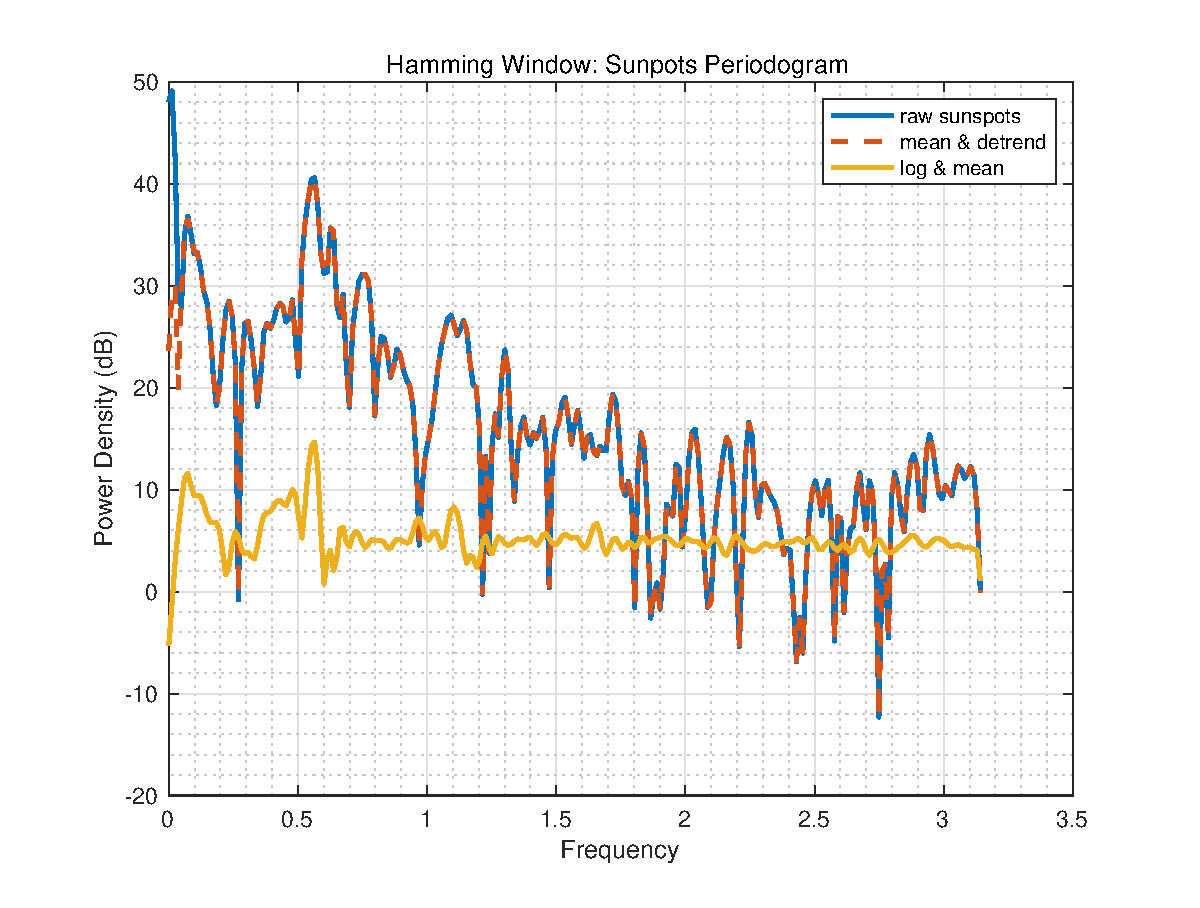
\includegraphics[height=1.5in]{Part1/1_2_a_2.eps}
    \caption{Sunspot time series: Hamming window periodogram method .}
    \label{fig:1_2_a}
\end{figure}
b) Figure \ref{fig:1_2_b_1}, is the standard and Bartlett periodogram of EEG data. The peaks are 8-10 Hz, 13 Hz, 26 Hz, 39 Hz, 50 Hz. The latter plots give the Bartlett method. 
According to the instructions in the booklet, 8-10 Hz is not SSVEP since it is tired while recording.The fundamental harmonic frequency of SSVEP is  at peak of 13 Hz and it is less visible as window length decreased. The first harmonic frequency of SSVEP is at 26 Hz, which is still visible as window length decreased. This may because there is no large interference near it. The second harmonic frequency of SSVEP is at 39 Hz, but it is less visible at lower window lengths. However, 50 Hz is not SSVEP because it has strong power-line-interference even at small window lengths. 

\begin{figure}[H]
    \centering
    \begin{subfigure}{0.35\textwidth}
        \centering
        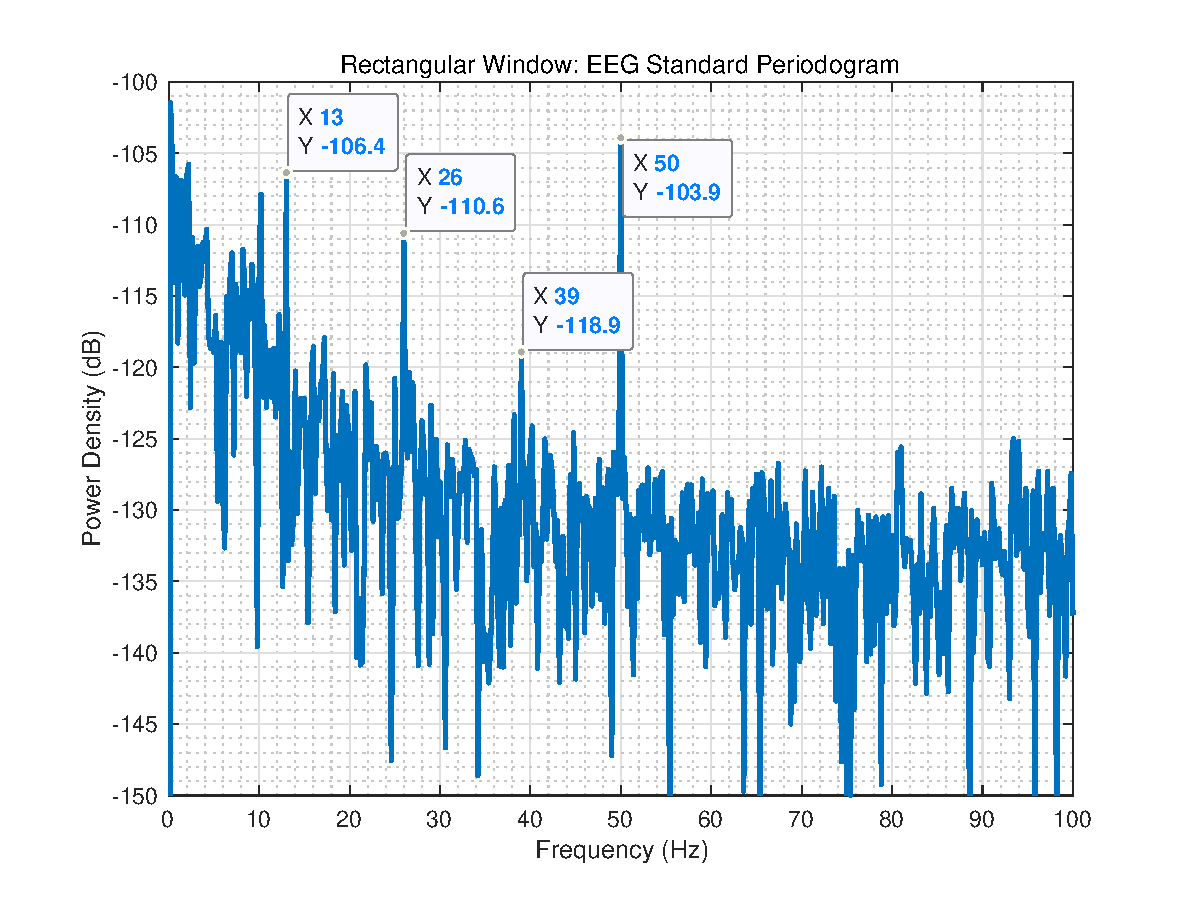
\includegraphics[height=1.5in]{Part1/1_2_b_1.eps}
    \end{subfigure}
    ~ 
    \begin{subfigure}{0.35\textwidth}
        \centering
        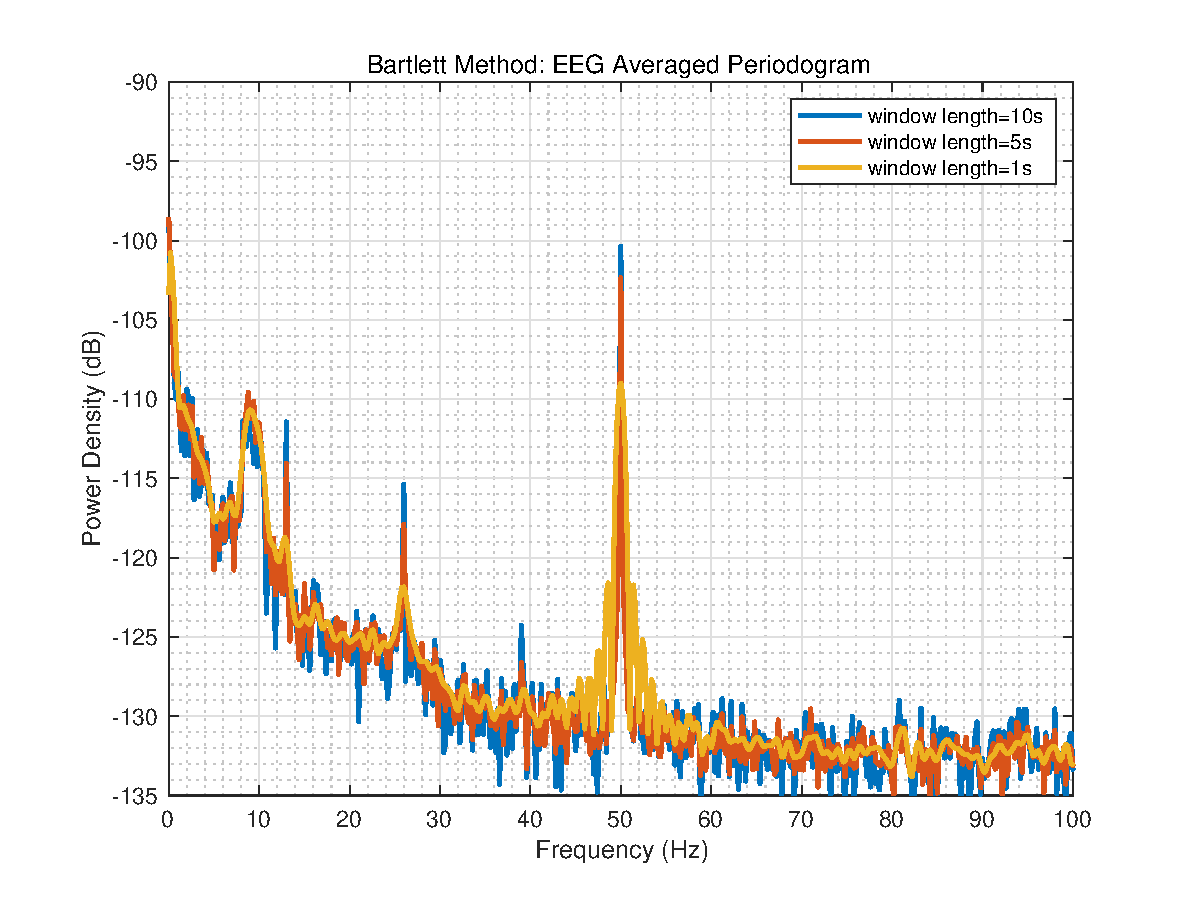
\includegraphics[height=1.5in]{Part1/1_2_b_2.eps}
    \end{subfigure}
    \caption{EEG samples: standard and Bartlett method periodogram with rectangular window .}
    \label{fig:1_2_b_1}
\end{figure}

\ref{fig:1_2_b_2} given the comparison of standard periodogram and averaged periodogram with 10s and 1s window length. It can be seen that as the window lengths become smaller, the components in 8-10 Hz can be still observed adequately.  Theoretically, as window length decreases, the number of captured periodograms increases and the variance decreases. However, the drawback is the frequency resolution also decreases. 
At window length is 10s, it can be seen that, the variance has slightly decreased but the resolution keep unchanged. The later figure with window length 1s, compared with 10s, it has a more reduced variance, but the resolution at peak 39 Hz has lost.
In conclusion, there is a trade-off between frequency resolution and variance minimizing. The situation varies from largest variance and precised resolution for standard periodograms to smallest variance but worst resolution for averaging periodogram with window size only 1s. 
\begin{figure}[H]
    \centering
    \begin{subfigure}{0.35\textwidth}
        \centering
        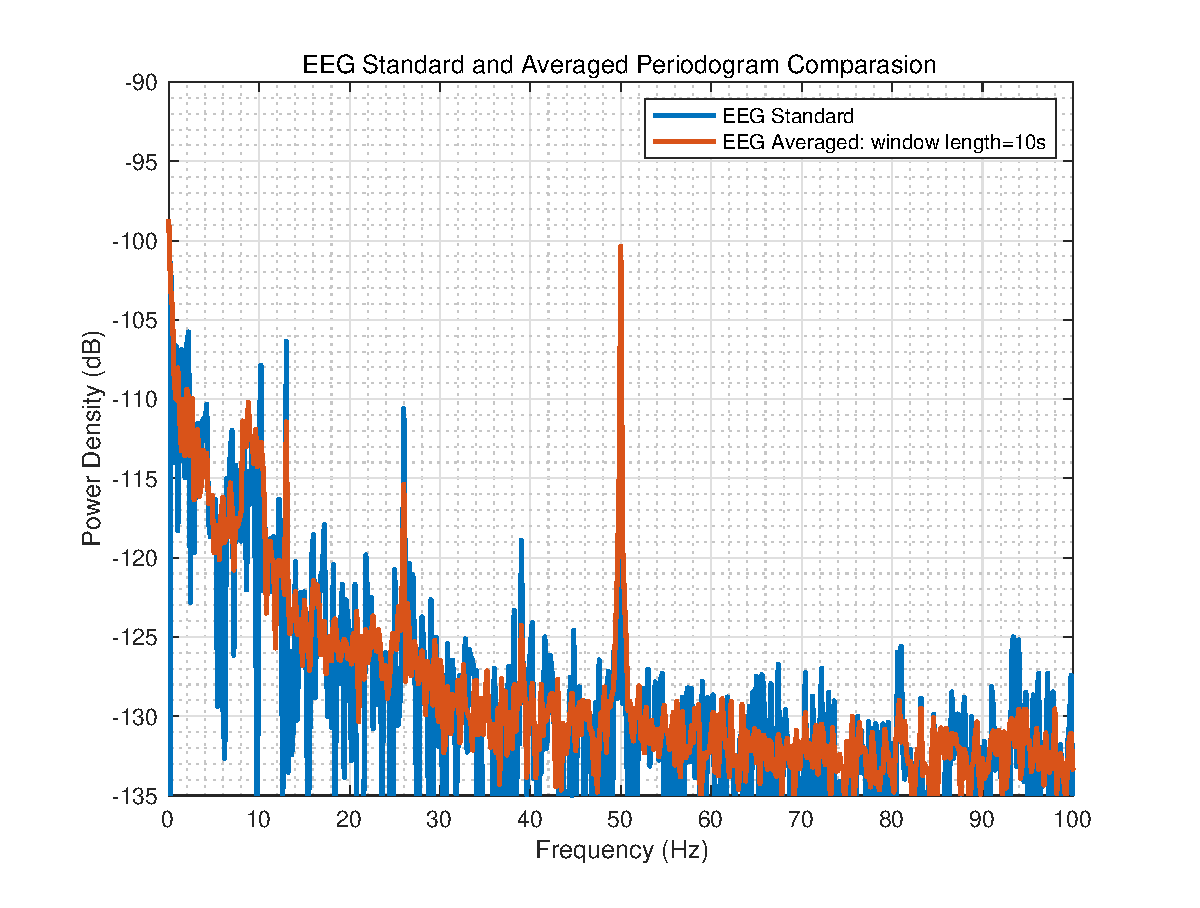
\includegraphics[height=1.5in]{Part1/1_2_b_3.eps}
    \end{subfigure}
    ~ 
    \begin{subfigure}{0.35\textwidth}
        \centering
        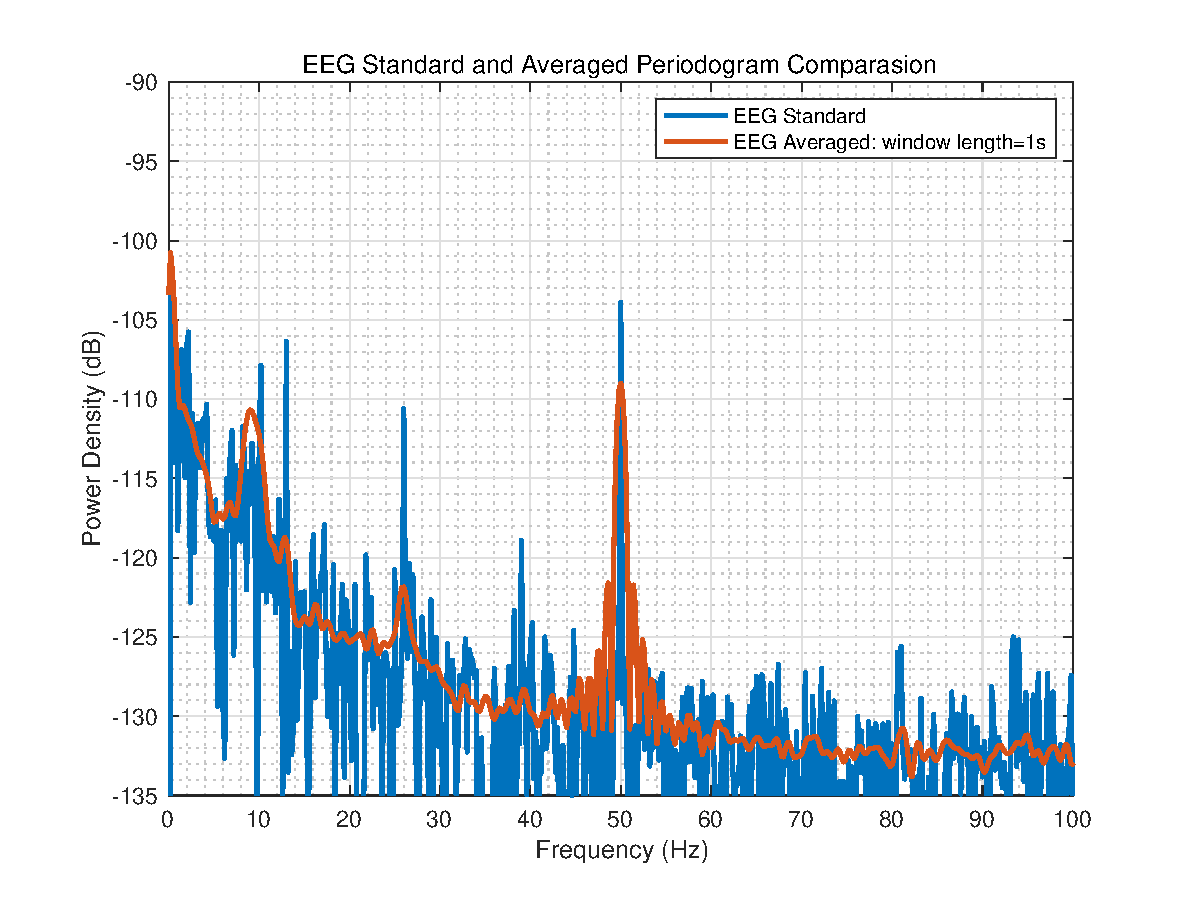
\includegraphics[height=1.5in]{Part1/1_2_b_4.eps}
    \end{subfigure}
    \caption{EEG samples: standard periodogram and averaged  periodogram with of window length 10s and 1s}
    \label{fig:1_2_b_2}
\end{figure}

\section{Correlation Estimation}
a)
Here Figure \ref{fig:1_3_c} shows the biased and unbiased ACF estimation and corresponding correlation for signals like WGN, noisy sinusoidal and filtered WGN. .  
\begin{figure}[H]
    \centering
    \begin{subfigure}{0.35\textwidth}
        \centering
        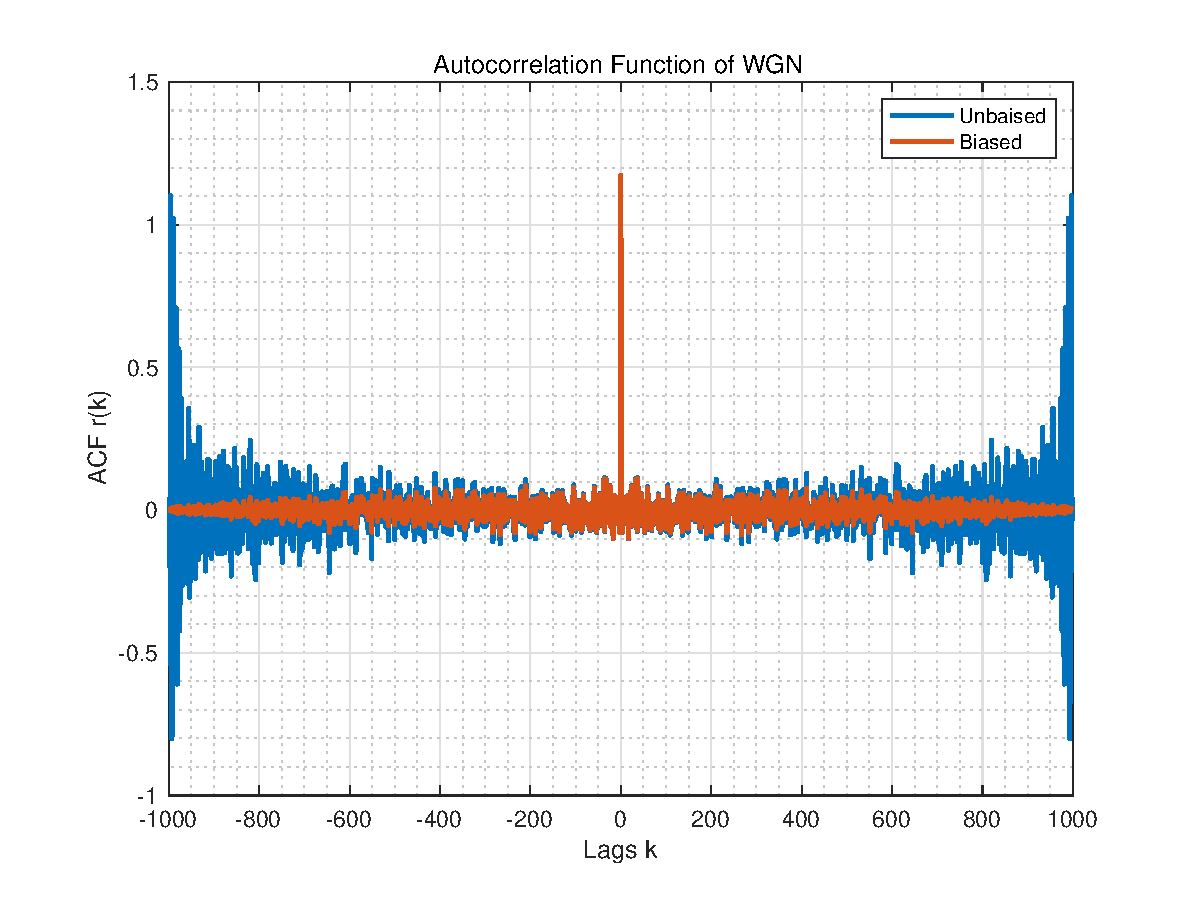
\includegraphics[height=1.5in]{Part1/1_3_a_1.eps}
    \end{subfigure}
    ~
    \begin{subfigure}{0.35\textwidth}
        \centering
        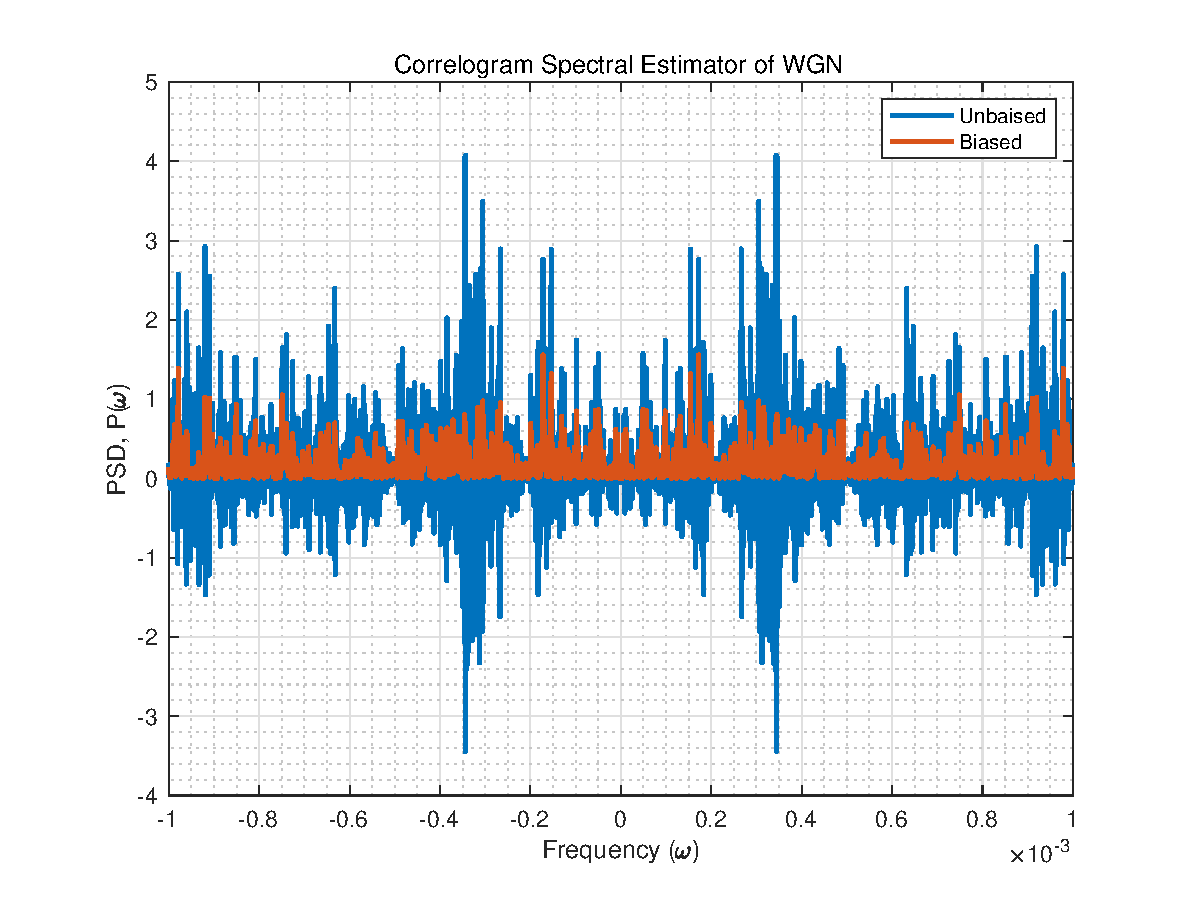
\includegraphics[height=1.5in]{Part1/1_3_a_2.eps}
    \end{subfigure}
    ~
    ~
    \begin{subfigure}{0.35\textwidth}
        \centering
        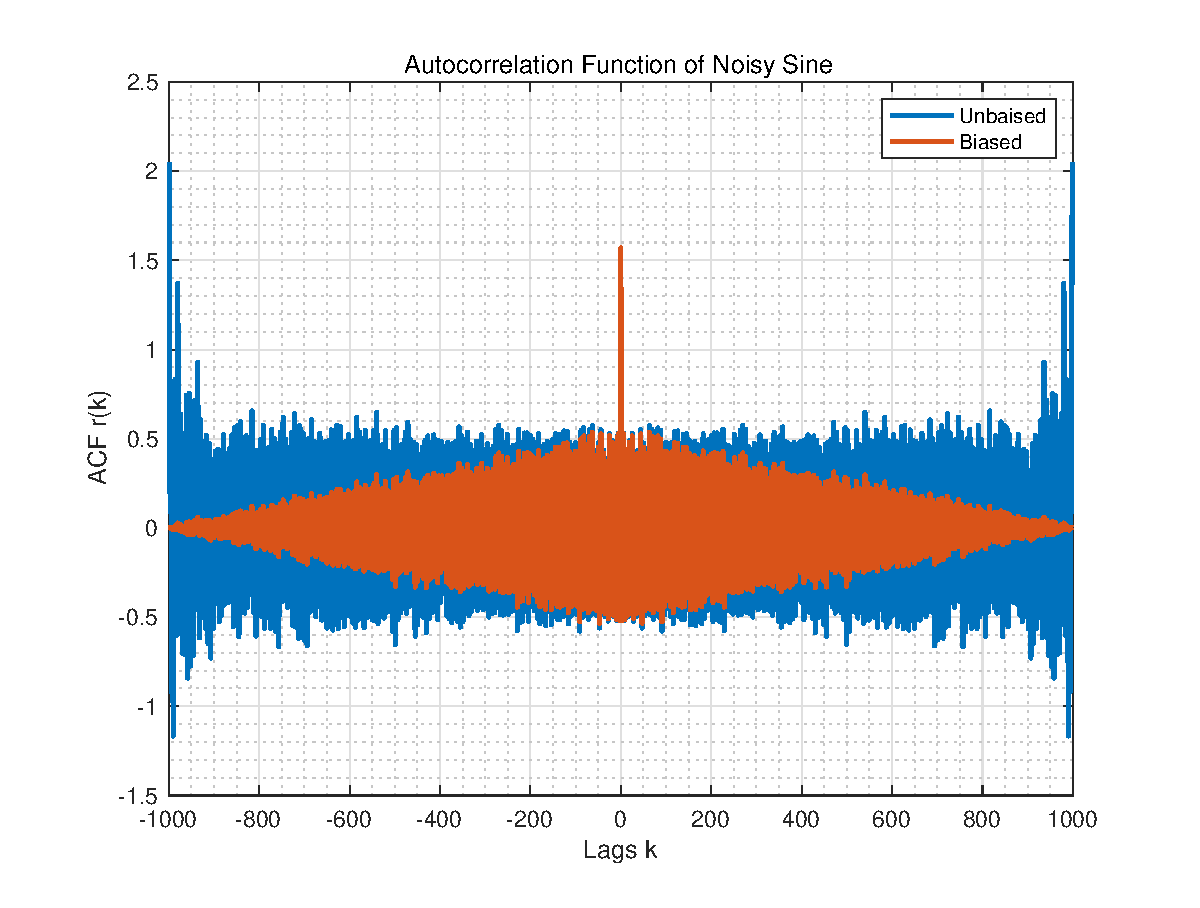
\includegraphics[height=1.5in]{Part1/1_3_a_nosiy1.eps}
    \end{subfigure}
    ~ 
    \begin{subfigure}{0.35\textwidth}
        \centering
        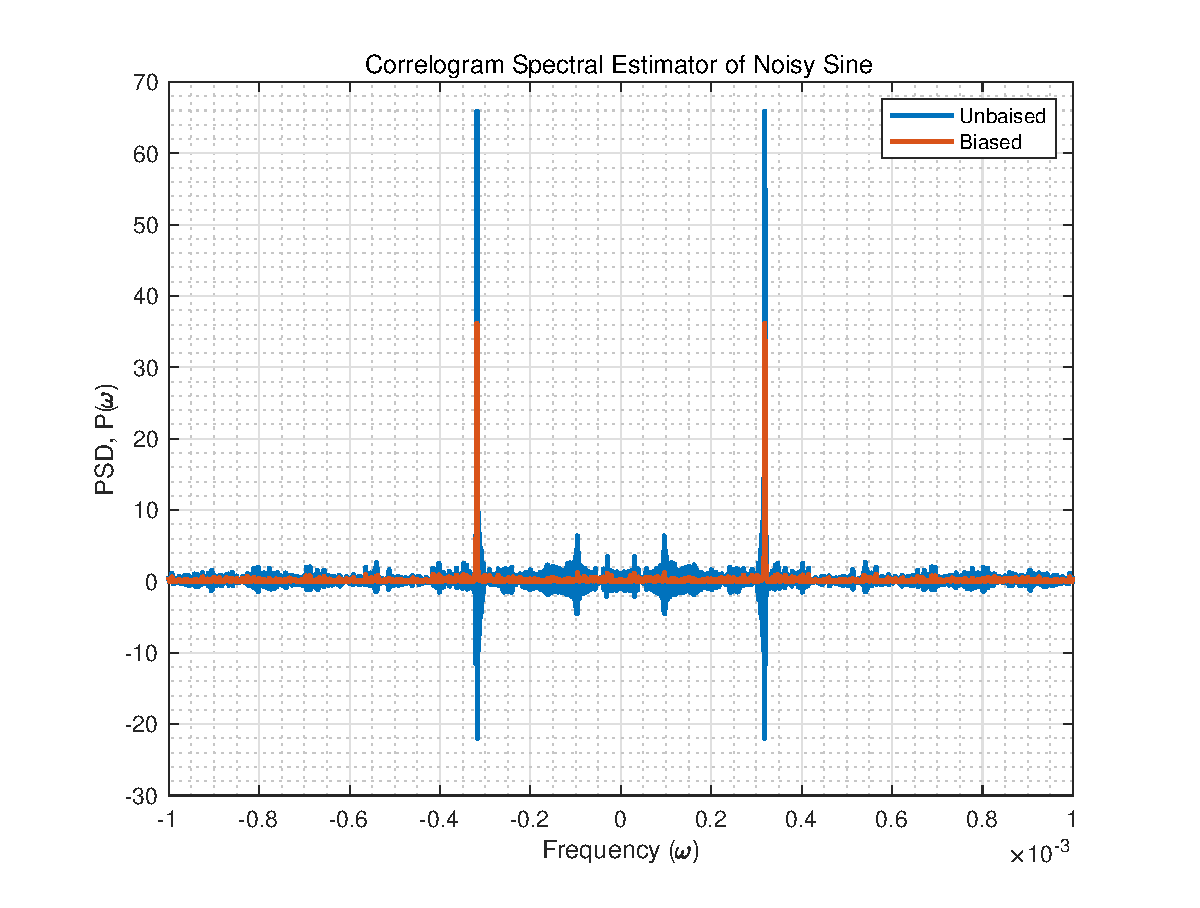
\includegraphics[height=1.5in]{Part1/1_3_a_nosiy2.eps}
    \end{subfigure}
    ~
    ~
    \begin{subfigure}{0.35\textwidth}
        \centering
        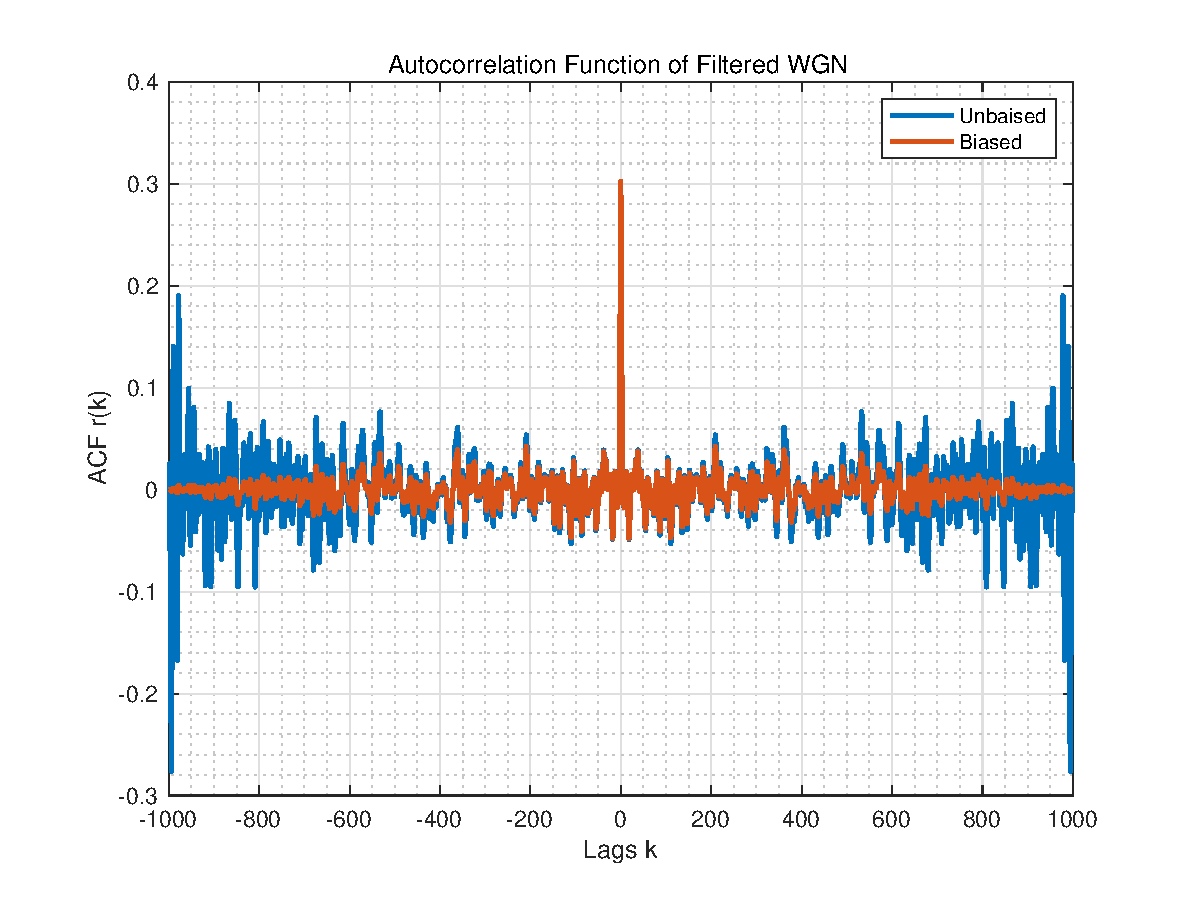
\includegraphics[height=1.5in]{Part1/1_3_a_wgn1.eps}
    \end{subfigure}
    ~
    \begin{subfigure}{0.35\textwidth}
        \centering
        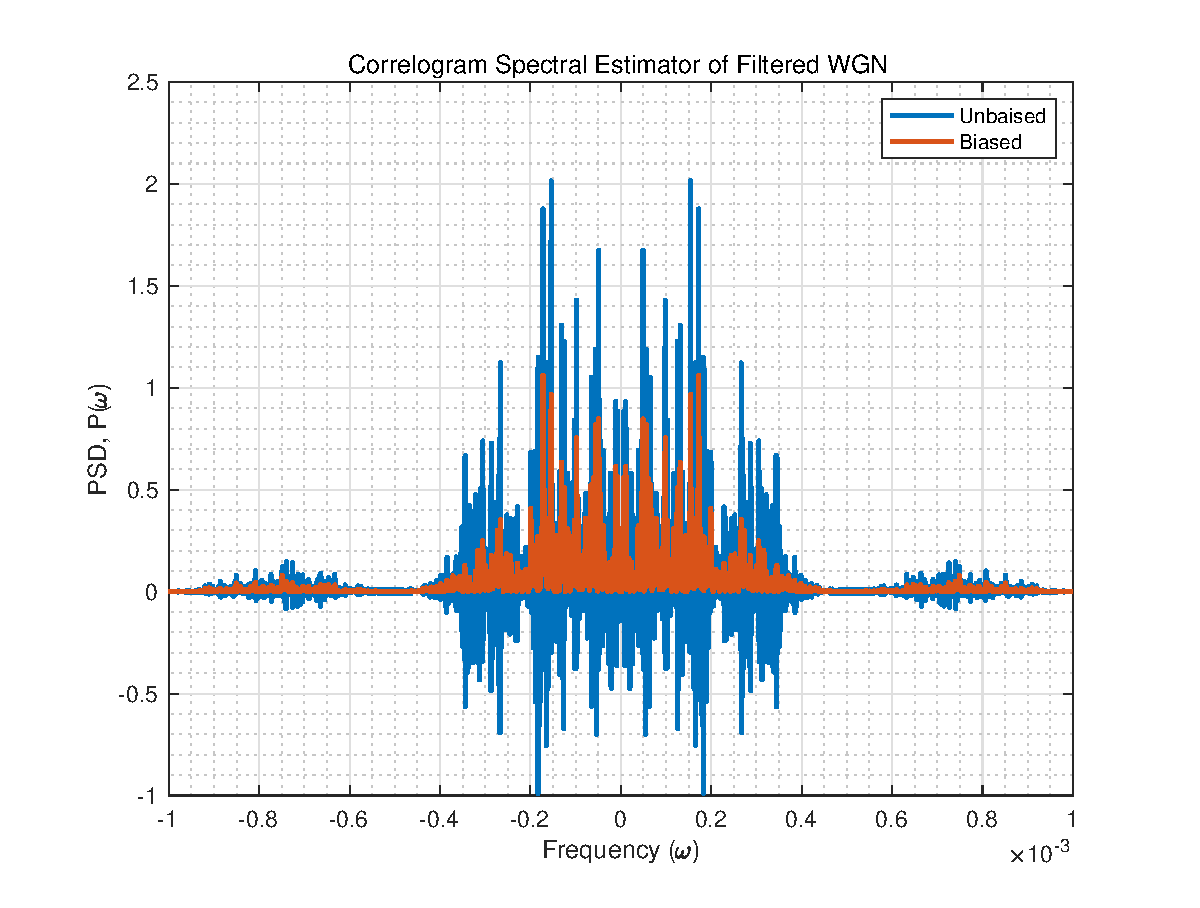
\includegraphics[height=1.5in]{Part1/1_3_a_wgn2.eps}
    \end{subfigure}
    \caption{ACF and Correlogram: biased and unbiased estimates of various signals.}
    \label{fig:1_3_a}
\end{figure}

b)

\begin{figure}[H]
    \centering
    \begin{subfigure}{0.35\textwidth}
        \centering
        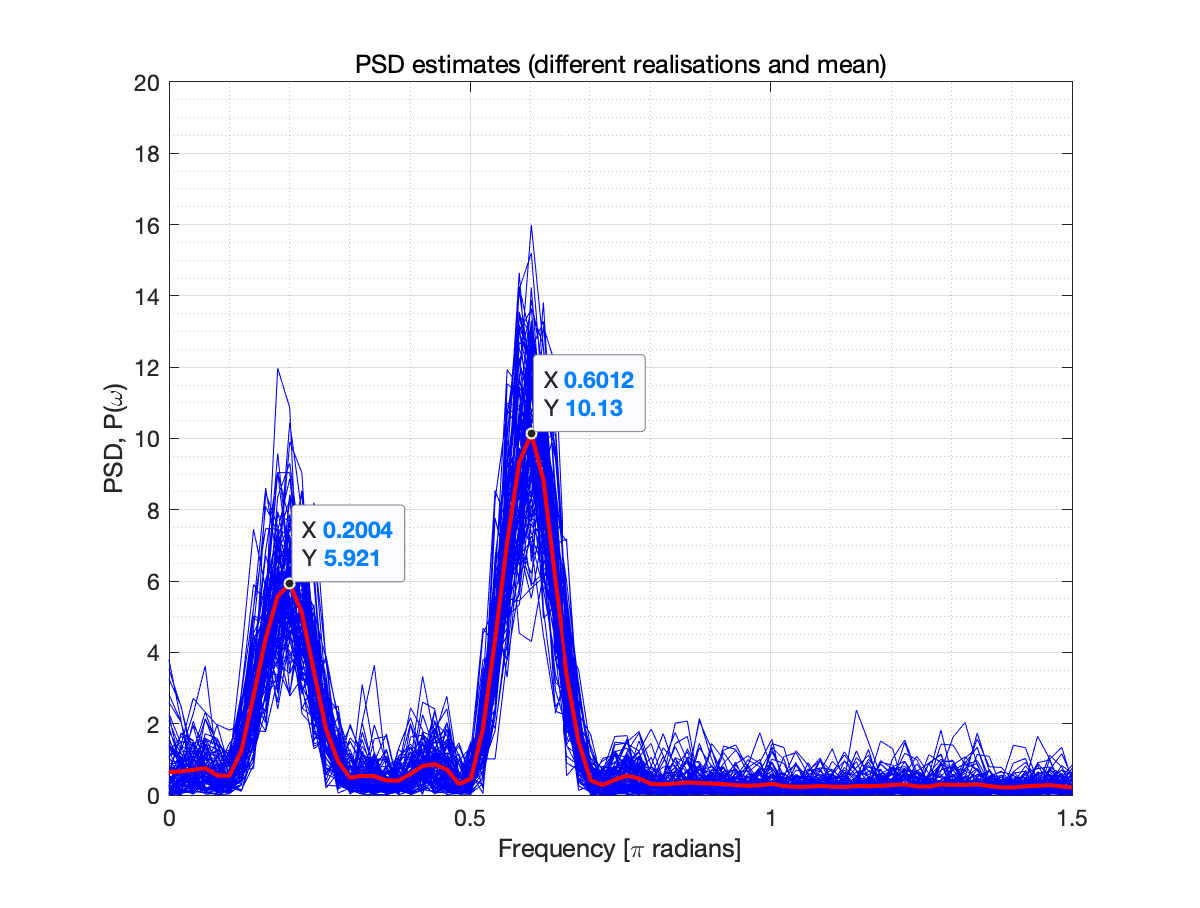
\includegraphics[height=1.5in]{Part1/1_3_b_1.eps}
    \end{subfigure}
    ~ 
    \begin{subfigure}{0.35\textwidth}
        \centering
        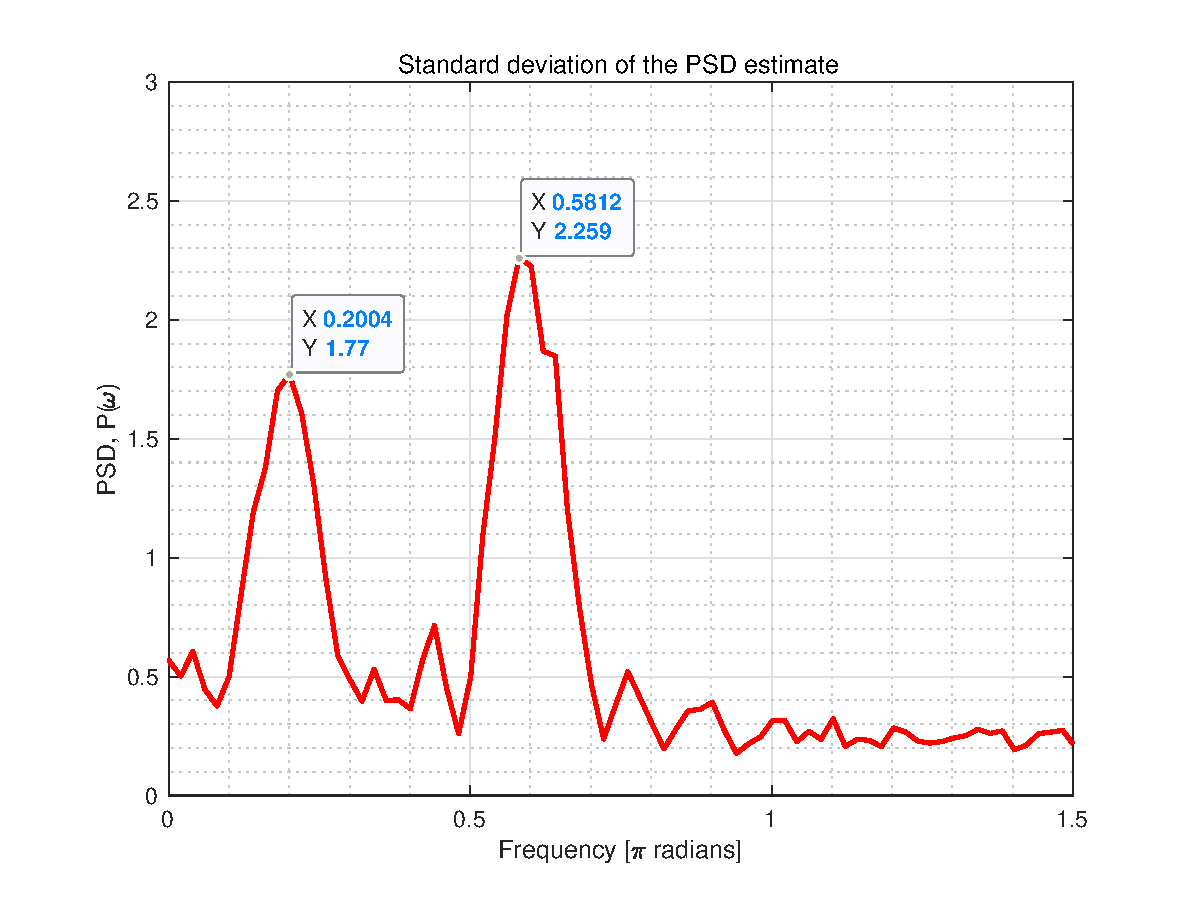
\includegraphics[height=1.5in]{Part1/1_3_b_2.eps}
    \end{subfigure}
    \caption{EEG samples: standard periodogram and averaged  periodogram with of window length 10s and 1s}
    \label{fig:1_2_b_2}
\end{figure}
c)
\begin{figure}[H]
    \centering
    \begin{subfigure}{0.35\textwidth}
        \centering
        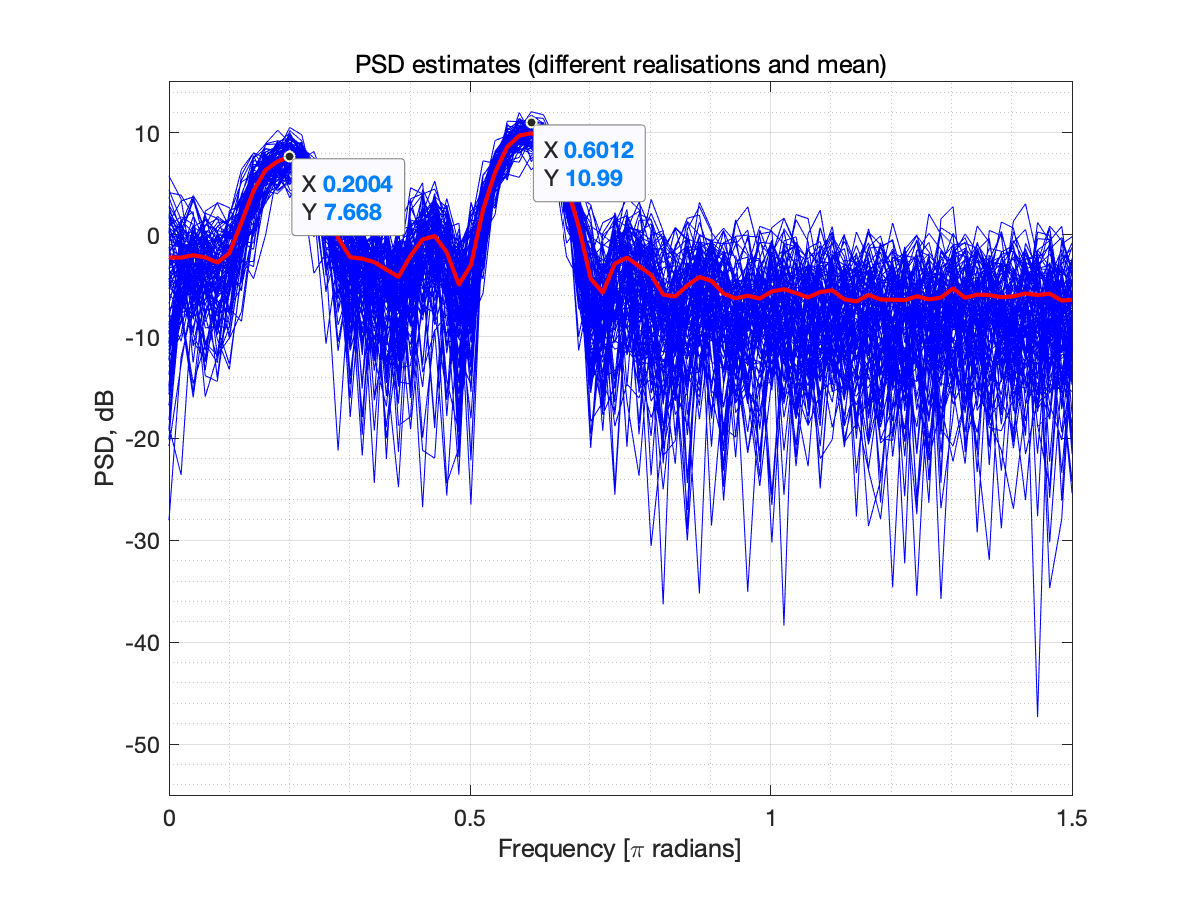
\includegraphics[height=1.5in]{Part1/1_3_c_1.eps}
    \end{subfigure}
    ~ 
    \begin{subfigure}{0.35\textwidth}
        \centering
        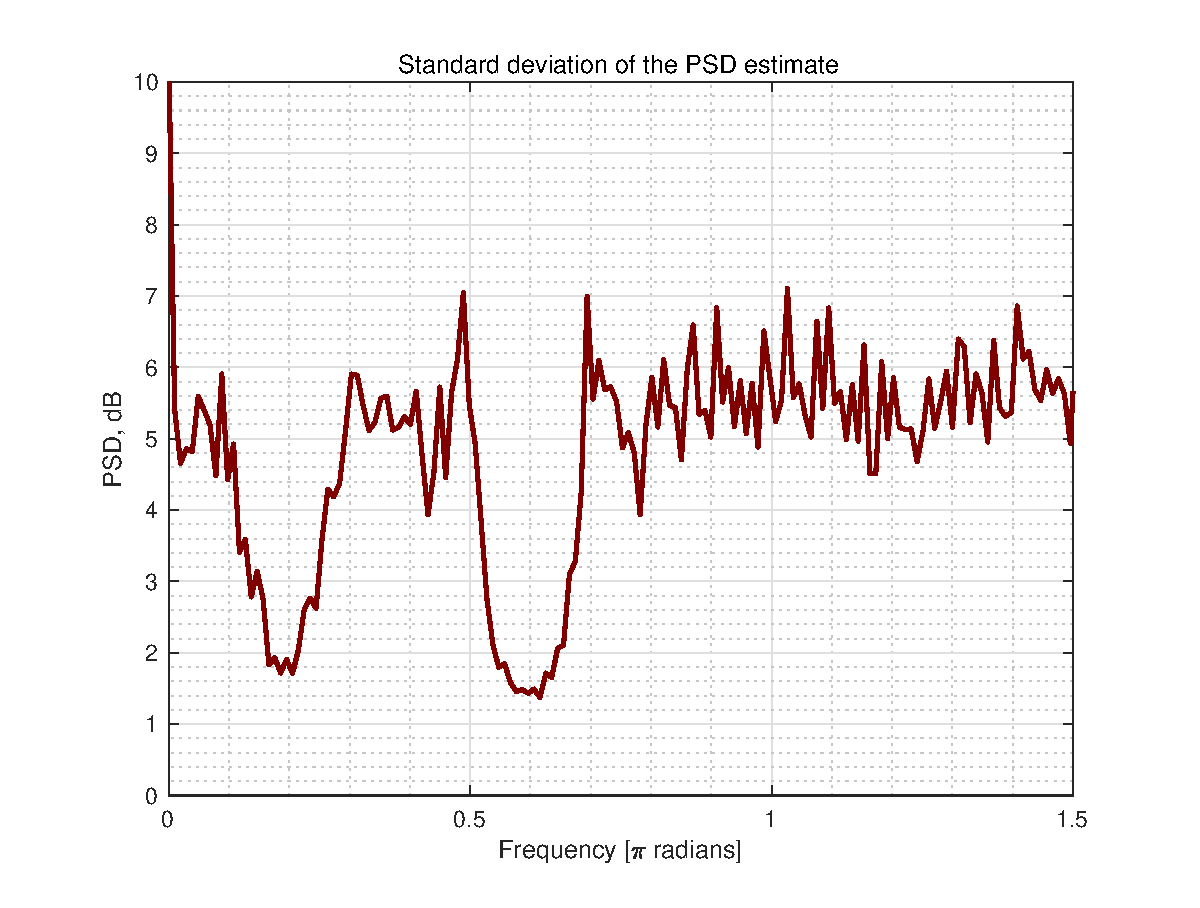
\includegraphics[height=1.5in]{Part1/1_3_c_2.eps}
    \end{subfigure}
    \caption{EEG samples: standard periodogram and averaged  periodogram with of window length 10s and 1s}
    \label{fig:1_3_c}
\end{figure}
d)

\begin{figure}[H]
    \centering
    \begin{subfigure}{0.35\textwidth}
        \centering
        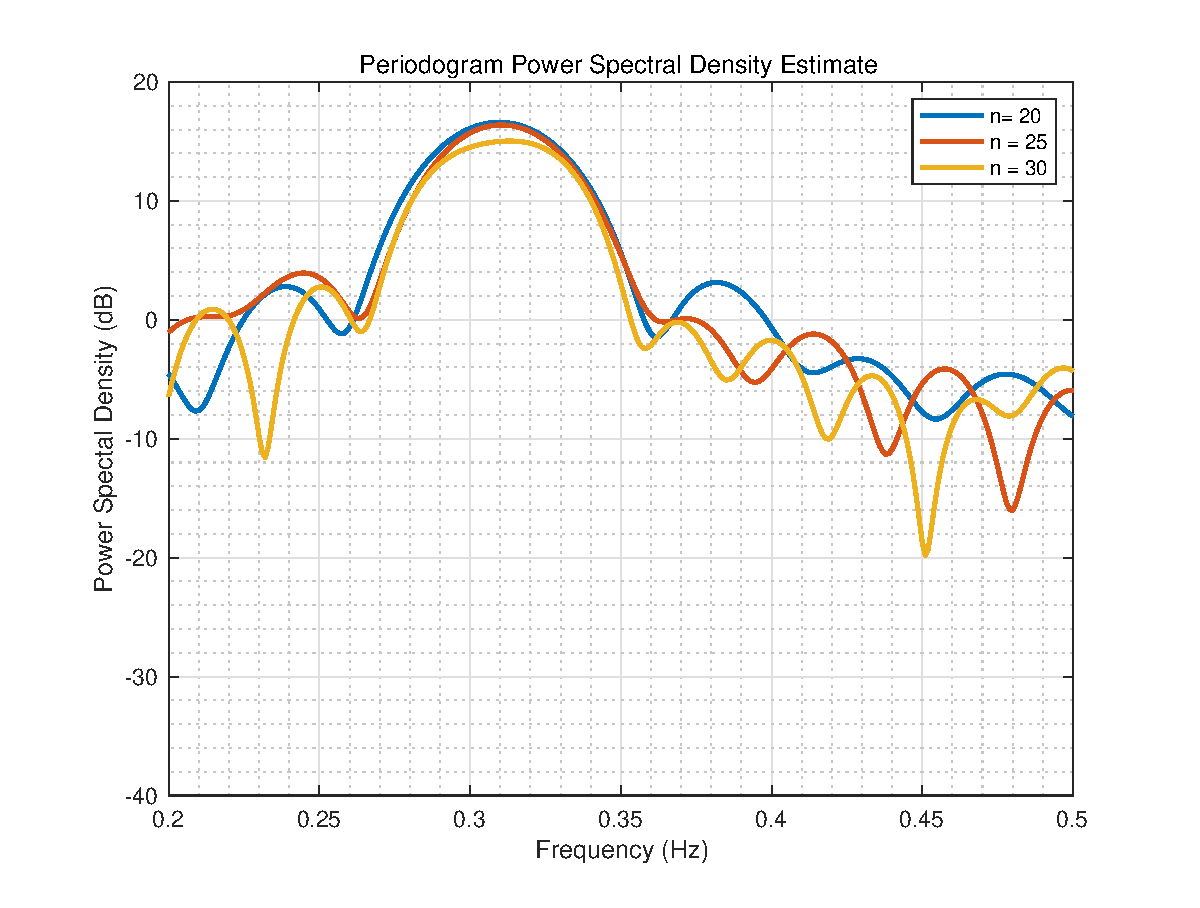
\includegraphics[height=1.5in]{Part1/1_3_d1.eps}
    \end{subfigure}
    ~ 
    \begin{subfigure}{0.35\textwidth}
        \centering
        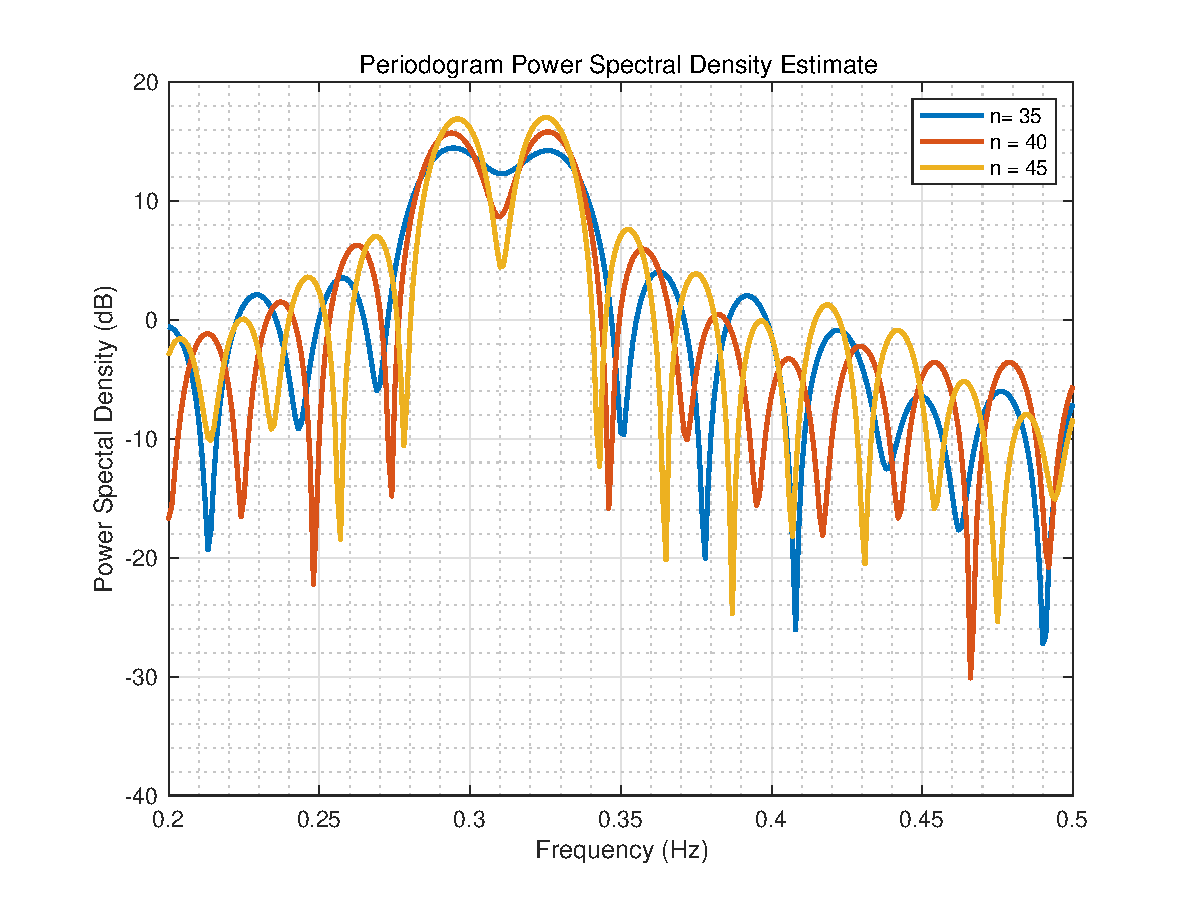
\includegraphics[height=1.5in]{Part1/1_3_d2.eps}
    \end{subfigure}
    \caption{EEG samples: standard periodogram and averaged  periodogram with of window length 10s and 1s}
    \label{fig:1_3_d_1}
\end{figure}
\begin{figure}[H]
    \centering
        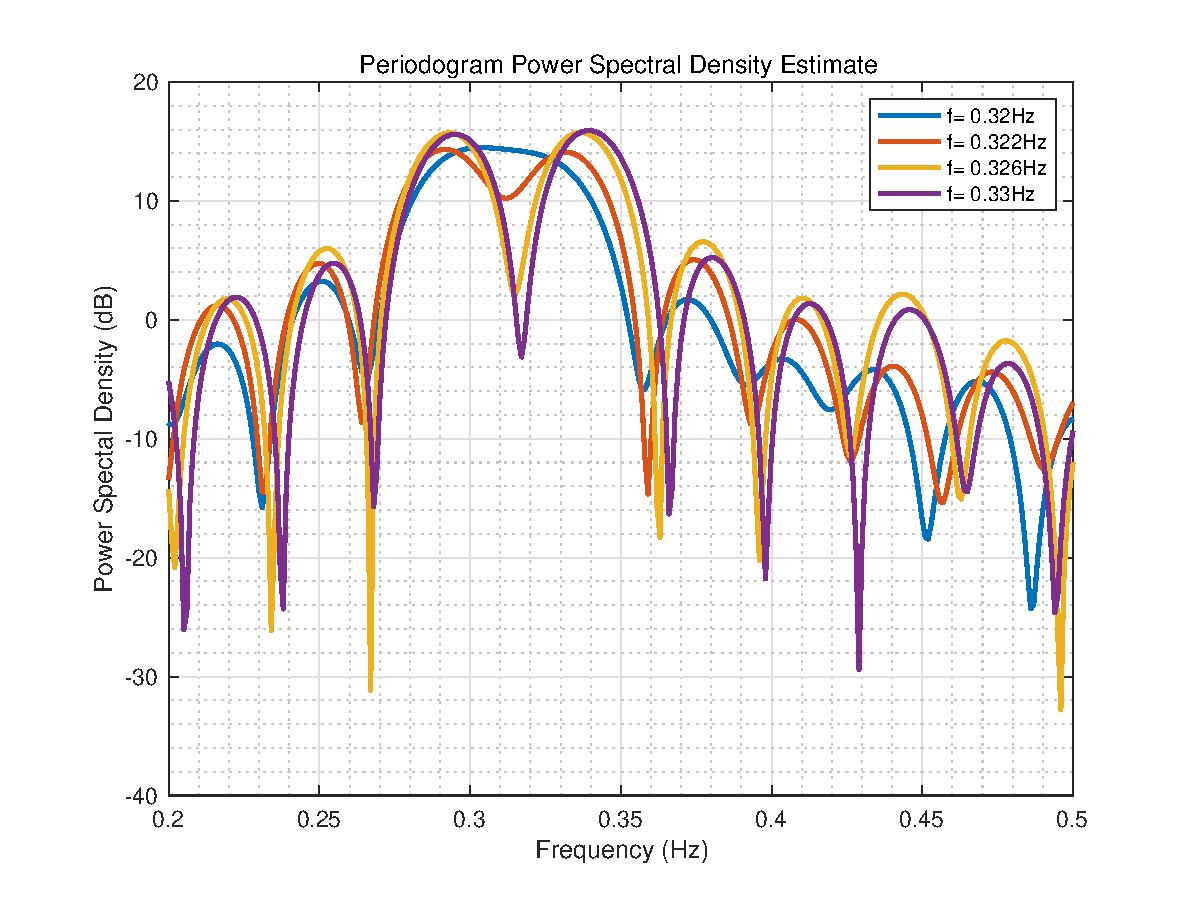
\includegraphics[height=1.5in]{Part1/1_3_d3.eps}
    \caption{Sunspot time series: Hamming window periodogram method .}
    \label{fig:1_3_d2}
\end{figure}
e)
\section{Spectrum of Autoregressive Processes}
%%a)
%% b)
%
\section{Real World Signals: Respiratory Sinus Arrhythmia from RR-Intervals}

\section{Robust Regression}


\chapter{Background}
\chapter{PROJECT X}
\chapter{Evaluation}
\chapter{Conclusion}
\appendix
\chapter{First Appendix}

\bibliographystyle{alpha}
\bibliography{bibs/sample}

\end{document}



